% A rough draft of the proof of the simple instruction reordering, given the memory model

%Some preliminary latex commands to format writing theorems 

\newtheorem{lemma}{Lemma}

\newtheorem{theorem}{Theorem}[lemma]

\newtheorem{corollary}{Corollary}[theorem]

\newtheorem{definition}{Definition}



\section{Instruction Reordering}
    One of the most common program transformations done by the compiler as well as the hardware is instruction reordering. The requirements for reordering in a sequential program is already well established and understood(cite). However, in a concurrent context, this is relatively less clear. 
    
    \paragraph{Simple reordering is not straightforward under shared memory semantics}
    One of the main aspects of programs using shared memory is the aspect of visibility of a memory write to different threads. The relaxed memory model of Javascript prescribe semantics for this using the $\stck{_{hb}}$ relations. Given this relation, it can be observed that seemingly "harmless" reordering using a sequential justification may not always keep the program behavior unchanged. 
    
    %GIVE ONE EXAMPLE BASED ON SEQUENTIALLY CONSISTENT WRITE/READ
    
    \paragraph{What can be done?}
    A simple example-based analysis, though would work for small programs become infeasible as the programs scale in length and complexity. It is also important to note that generalizations by using a small sample size is not something we can afford especially when we want to ensure these program trasnformations are automated contrast to being transformed manually.
    
    \subsection{Our approach}
    One solution to this is to construct a proof that would expose/specify the conditions under which reordering is possible. To keep things simple, we first consider when consecutive instructions can be reordered, followed by non-consecutive cases. The crux of the proof is to guarantee that reordering does not bring any new reads-from relations that did not exist in any execution of the original program. It is important to note however, that a proof in this sense would be generalized to any program , so often it might be the case that for specific programs, instruction reordering can be valid, however, in a general sense may not be valid for others. 
    
    %GIVE TWO EXAMPLES TO SHOW THIS. POSSIBLY USE THE EXAMPLE ABOVE AND EXPLAIN

%---------------------------------------------------------------------------------------------------------------------------------------    
    
    %Something we need to define for sake of proofs
    \begin{definition}{Consecutive pair of Events (\emph{cons})}
        
        We define \emph{cons} as a function, which takes two events as input, and gives us a boolean indicating if they are consecutive pairs. Two events $e$ and $d$ are consecutive if they have an $\stck{_{ao}}$ relation among them and are \emph{next to each other}, which can be defined formally as 
        
        \[
            cons(e,d) \ \Rightarrow \ 
            (
                e \stck{_{ao}} d  \ \wedge \ 
                \nexists k \ \textit{s.t.} \ 
                e \stck{_{ao}} k  \ \wedge \
                k \stck{_{ao}} d  \ \wedge \
            )
            \ \vee \
            (
                d \stck{_{ao}} e  \ \wedge \ 
                \nexists k \ \textit{s.t.} \ 
                d \stck{_{ao}} k  \ \wedge \
                k \stck{_{ao}} e  
            )
        \]
        
        \critic{blue}{Input space for \emph{cons} is the Cartesian product of Event set with itself}
        
    \end{definition}

%A new definition to define direct relations. This will help us concisely state our arguments in the proofs that will come henceforth
\begin{definition}{Direct happens-before Relation (dir)}
    
    We define \textit{dir} that takes an ordered pair of events $(e,d)$ such that $\reln{e}{hb}{d}$ and gives a boolean value to indicate whether this relation is \textit{direct}. By \textit{direct}, we mean those relations that are not derived through transitive property of $\stck{_{hb}}$.
    
    We can infer certain things using this function based on some information on events $e$ and $d$. 
    \begin{itemize}
        \item If $\et{e}{uo}$, then $dir(e,d) \ \Rightarrow \ cons(e,d)$
        \item If $\et{d}{uo}$, then $dir(e,d) \ \Rightarrow \ cons(e,d)$
        \item If $\et{e}{sc} \wedge e\!\in\!R$, then $dir(e,d) \ \Rightarrow \ cons(e,d)$
        \item If $\et{e}{sc} \wedge e\!\in\!W$, then $dir(e,d) \ \Rightarrow \ cons(e,d) \vee \reln{e}{sw}{d}$
        \item If $\et{d}{sc} \wedge d\!\in\!W$, then $dir(e,d) \ \Rightarrow \ cons(e,d)$
        \item If $\et{d}{sc} \wedge e\!\in\!R$, then $dir(e,d) \ \Rightarrow \ cons(e,d) \vee \reln{e}{sw}{d}$
    \end{itemize}


\end{definition}


%A new command to quickly use cons function in formal descriptions
\newcommand{\cons}[2]{\textit{cons}(#1,#2)}
  
%--------------------------------------------------------------------------------------------------------------   
    \subsection{Lemmas to assist our proof}    
    In order to assist our proof, we define two \textit{lemmas} based on the ordering relations. 
    
    \begin{lemma} Consider three events $e$,$d$ and $k$. \\
    
        If
            \[
                \cons{e}{d} \ \wedge \ \reln{e}{ao}{d} \ \wedge \
                (
                    (\et{d}{uo}) \ \vee \
                    (\et{d}{sc} \ \wedge \ \event{d}{W})
                )
            \]
            
        then,
            \[
                \reln{k}{hb}{d} \Longrightarrow \reln{k}{hb}{e}
            \]
          
        When we have two consecutive events \textit{e} and \textit{d} which are one after the other (i.e. $\reln{e}{ao}{d}$), we can use \textit{transitive property} of $\stck{_{hb}}$ to infer that any event \textit{k} that \textit{happens before} \textit{e}, also \textit{happens before} \textit{d}. However, is it possible to derive that the event \textit{k happens before e} using the evidence that \textit{k happens before d} ? This lemma states the condition when this is true.
        
    \end{lemma}
    
    %An alternative short proof 
    \begin{proof}
        
        We will divide the proof for this into two cases, based on what event $d$ is. For both cases, we have the following to be true :
        
        \[
            cons(e,d) \ \wedge \ \reln{e}{ao}{d}
            \tag{0}
            \label{l10}
        \]
    
        In the first case, 
        
        \[
            \et{d}{uo} 
            \tag{1}
            \label{l11}
        \]
        
        Then for any event $k$
        \[
            dir(k,d) \Rightarrow cons(k,d)
            \qquad from \quad
            (\ref{l11})
            \tag{2}
            \label{l12}
        \]
        
        The event that has such a relation with $d$ is $e$.
        \[
             k = e  
             \qquad from \quad
             (\ref{l10}, \ref{l12})
             \tag{3}
             \label{l13}
        \]
        
        Because $\stck{_{ao}}$ is a total order, $e$ will be the only event. This would mean that for any other $k \neq e$,
        
        \[
            \reln{k}{hb}{d} \Rightarrow \reln{k}{hb}{d}
            \qquad from \quad
            (\ref{l10}, \ref{l11}, \ref{l12}, \ref{l13}) 
        \]
        
        The following figure should explain this intuition:  
        \begin{figure}[H]
            \centering
            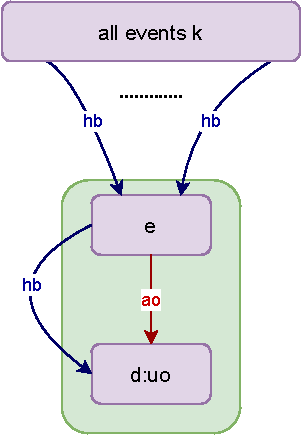
\includegraphics[scale=0.7]{Lemma_Proof1_Case1.pdf}
            \caption{For the first case}
            \label{fig:my_label}
        \end{figure}
        
        In the second case,
        \[
            \et{d}{sc} \wedge d\!\in\!W
            \tag{4}
            \label{l14}
        \]
        
        Then for any event $k$
        \[
            dir(k,d) \Rightarrow cons(k,d)
            \qquad from \quad
            (\ref{l14})
            \tag{5}
            \label{l15}
        \]
        
        We once again have event $e$ having such a relation 
        \[
            k = e 
            \qquad from \quad
            (\ref{l10}, \ref{l15})
            \tag{6}
            \label{l16}
        \]
        
        Though there could be direct \textit{happens-before} relation with some event $k$ from another \textit{agent}, these are only relations satisfying $dir(d,k)$. Thus, we can once again infer that for any $k \neq e$ 
        
        \[
            \reln{k}{hb}{d} \Rightarrow \reln{k}{hb}{d}
            \qquad from \quad
            (\ref{l10}, \ref{l14}, \ref{l15}, \ref{l16})
        \]
        
        The following figure explains this intuition: 
        
        \begin{figure}[H]
            \centering
            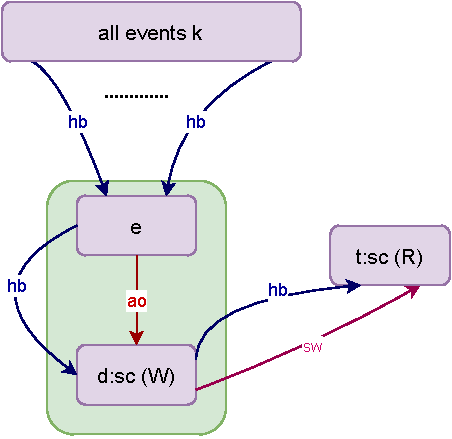
\includegraphics[scale=0.7]{Lemma_Proof1_Case2.pdf}
            \caption{For the second case}
            \label{fig:my_label}
        \end{figure}
        
    \end{proof}
    
%---------------------------------------------------------------------------------------------------------------    
    
%SHORTER VERSION OF PROOF WITHOUT THE ENGLISH EXPLAINATION IN THE MIDDLE. DISCUSS AND DECIDE ON WHICH FORM IS BETTER
    \begin{lemma}Consider three events $e$, $d$ and $k$ \\
    
        If
            
            \[
                \cons{e}{d} \ \wedge \ \reln{e}{ao}{d} \ \wedge \
                (
                    (\et{e}{uo}) \ \vee \
                    (\et{e}{sc} \ \wedge \ \event{e}{R})
                )
            \]
            
        then,
            \[
                \reln{e}{hb}{k} \Longrightarrow \reln{d}{hb}{k}
            \]
    
     When we have two consecutive events \textit{e} and \textit{d} which are one after the other (i.e. $\reln{e}{ao}{d}$), we can use \textit{transitive property} of $\stck{_{hb}}$ to infer that any event \textit{k} that \textit{happens after} \textit{d}, also \textit{happens after} \textit{e}. However, is it possible to derive that the event \textit{k happens after d} using the evidence that \textit{k happens after e} ? This lemma states the condition when this is true.
    
    \end{lemma}
    
    %An alternative proof for this 
    \begin{proof}
        
        Just like the proof for the previous lemma, we will divide the proof for this into two cases, based on what event $e$ is. Again, for both cases, we have the following to be true:
        
        \[
            cons(e,d) \ \wedge \reln{e}{ao}{d}
            \tag{0}
            \label{l20}
        \]
    
       In the first case,
       
       \[
            \et{e}{uo} 
            \tag{1}
            \label{l21}
       \]
       
       Then for any event k
       
       \[
            dir(e,k) \Rightarrow cons(e,k) 
            \qquad from
            \quad (\ref{l21})
            \tag{2}
            \label{l22}
       \]
       
       The event that has such a relation with $e$ is $d$
       \[
            k = d 
            \qquad from 
            \quad (\ref{l20}, \ref{l22})
            \tag{3}
            \label{l23}
       \]
       
       Because $\stck{_{ao}}$ is a total order, $d$ would be the only such event. This would mean that for any other event $k \neq d$
       
       \[
            \reln{e}{hb}{k} \Rightarrow \reln{d}{hb}{k}
            \qquad from 
            \quad (\ref{l20}, \ref{l21}, \ref{l22}, \ref{l23})
       \]
       %Better phrase the intuition
       The following figure should explain this intuition:  
        
        \begin{figure}[H]
            \centering
            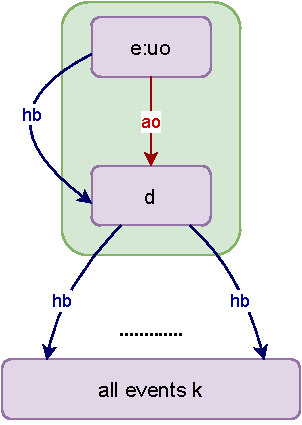
\includegraphics[scale=0.7]{Lemma_Proof2_Case1.pdf}
            \caption{Caption}
            \label{fig:my_label}
        \end{figure}
        
        In the second case,
        \[
            \et{e}{sc} \wedge e\!\in\!R
            \tag{4}
            \label{l24}
        \]
        
        Then for any event $k$
        \[
            dir(e,k) \Rightarrow cons(e,k)
            \qquad from \quad
            (\ref{l24})
            \tag{5}
            \label{l25}
        \]
        
        We once again have event $e$ having such a relation 
        \[
            k = d 
            \qquad from \quad
            (\ref{l20}, \ref{l25})
            \tag{6}
            \label{l26}
        \]
        
        Though there could be direct \textit{happens-before} relation with some event $k$ from another \textit{agent}, these are only relations satisfying $dir(k,e)$. Thus, we can once again infer that for any $k \neq d$ 
        
        \[
            \reln{e}{hb}{k} \Rightarrow \reln{d}{hb}{k}
            \qquad from \quad
            (\ref{l10}, \ref{l24},  \ref{l25}, \ref{l16})
        \]
        
        The following figure explains this intuition: 
        
        \begin{figure}[H]
            \centering
            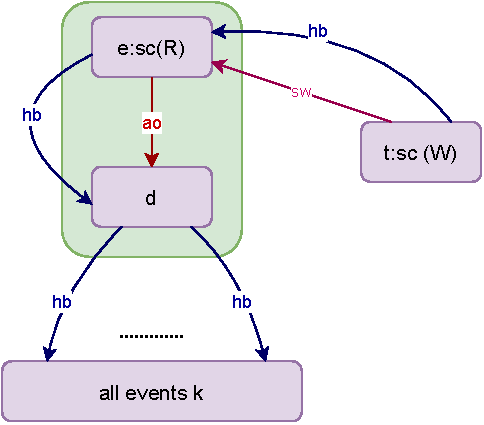
\includegraphics[scale=0.7]{Lemma_Proof2_Case2.pdf}
            \caption{Caption}
            \label{fig:my_label}
        \end{figure}

    \end{proof}
    
%Uptil here, it should be constant. Henceforth, we need to start writing/ changing
%------------------------------------------------------------------------------

\subsection{Abstract view of reordering}
    
    We view reordering as manipulating the agent-order relation among two events. In that sense, reordering two consecutive events $e$ and $d$ such that $e \stck{_{ao}} d$ becomes:
    \[
        e \stck{_{ao}} d 
        \longmapsto
        d \stck{_{ao}} e 
    \]
    
    What implications this change has on the other ordering relations depends on the type of events $e$ and $d$ are. The main relations we would want to retain would be those described by $\stck{_{hb}}$. The intuition is that the axioms of the memory model rely mainly on this ordering relation to restrict observable behaviors in a program. It is important to note that this is a conservative assertion to ensure reordering is safe, and by no means does it say that one cannot reorder otherwise. There could be certain examples of programs that would not harm when certain reordering is done, but in a general sense, this may not be true for all possible programs. 
    
    In the end, we want to ensure that the set of possible observable behaviors of a program, remain unchanged after reordering. If that is not feasible, then we would want the set of observable behaviors after reordering at the very least to be a subset. This would ensure that the program does not have some new behaviours that weren't supposed to happen prior to reordering. 
    
    \critic{red}{One might wonder what about the $\stck{_{mo}}$ relation. The intuition for us is that memory order, though it plays a role in the observable behaviors, only influences the observable behaviors when considering all sequentially consistent events. (refer to the last axiom of the memory model). In addition to this, memory order plays a role only with events having equal range that conflict.  Otherwise, every other axiom, necessarily relies on $\stck{_{hb}}$ relation. Of course, the tear-free axiom does not involve any ordering relations, but since we are not changing the tearing aspect of events during reordering, that aspect does not concern our proof.}

\subsection{Valid reordering}

    \begin{definition}{Reorderable Pair (Reord)}
        We define a boolean function \emph{Reord} that takes two ordered pair of events $e$ and $d$ such that $\reln{e}{ao}{d}$ and gives a boolean value indicating if they are a reorderable pair. 
        
         \begin{align*}
            Reord(e,d) = \\
            (
            ((\et{e}{uo} \wedge \et{d}{uo}) \ \wedge \\ 
                \quad ( 
                        &(\event{e}{R} \wedge \event{d}{R}) \vee \\ 
                        &(\event{e}{W} \wedge \event{d}{R} \wedge (\Re(e) \And \Re(d) = \phi)) \vee \\
                        &(\event{e}{R} \wedge \event{d}{W} \wedge (\Re(e) \And \Re(d) = \phi)) \vee \\
                        &(\event{e}{W} \wedge \event{d}{W} \wedge (\Re(e) \And \Re(d) = \phi)) 
                    )
            ) \\ \vee \\
            ((\et{e}{sc} \wedge \et{d}{uo}) \ \wedge \\
                \quad (
                        & (\event{e}{W} \wedge \event{d}{R} \wedge (\Re(e) \And \Re(d) = \phi)) \vee \\
                        & (\event{e}{W} \wedge \event{d}{W} \wedge (\Re(e) \And \Re(d) = \phi)) 
                    )
            ) \\ \vee \\
            ((\et{e}{uo} \wedge \et{d}{sc}) \ \wedge \\
                \quad (
                        & (\event{e}{R} \wedge \event{d}{R} \wedge) \vee \\
                        & (\event{e}{W} \wedge \event{d}{R} \wedge (\Re(e) \And \Re(d) = \phi)) 
                    )
            )
            )
    \end{align*}
    \end{definition}

\begin{theorem} 

    Consider a candidate $C$ of a program and its \textit{Candidate Executions} which are valid. Consider two events $e$ and $d$ such that $\cons{e}{d}$ is true in $C$ and  $\reln{e}{ao}{d}$. Consider another candidate $C'$ resulting after reordering $e$ and $d$. 
    Then if \emph{Reord(e,d)} is true in $C$, the set observable behaviors possible in $C'$ is a subset of that of $C$. 
\end{theorem}

\begin{proof}

    The proof is structured as follows. We first show that existing \textit{happens-before} relations in any candidate execution of $C$ except $\reln{e}{hb}{d}$ remain intact after reordering. We then identify the cases where new \textit{happens-before} relations could be established. We then show that these new relations do not introduce any new observable behaviors. Lastly, we identify from the remaining cases whether \textit{happens-before} cycles could be introduced.
    
    The above steps can be summarized as addressing four main questions for any $Candidate Execution$ of $C'$
    \begin{enumerate}
        \item Apart from the events involved in reordering, do other \emph{happens-before} relations remain intact?
        \item Are any new \emph{happens-before} relations established? 
        \item Do they new relations bring new \emph{observable behaviors?}
        \item Are any \emph{happens-before} cycles introduced? 
    \end{enumerate}
    
    %The first two questions ensure that existing happens-before relations are intact
    
    \paragraph{1. Preserving \textit{happens-before} relations}
        
        If some $\stck{_{hb}}$ relations among events are lost after reordering, we may introduce new observable behaviors. So the first step is to ensure that the existing relations in any Candidate Execution of $C$ remain preserved after reordering, thus showing that the new Candidate Execution due to $C'$ has the previous relations preserved. 
        
        \critic{blue}{The intuition is that if all the other $\stck{_{hb}}$ relations are intact, the axioms that rely on this relation will not place more restrictions on possible $\stck{_{rf}}$ relations.} 
        
        The relations that could be subject to change can be addressed by considering two disjoint sets of events in any \textit{Candidate Execution} of $C$ as below.
        
        \[
            K_e = \{k \ | \ \reln{k}{hb}{e} \}
        \]
        
        \[
            K_d = \{k \ | \ \reln{d}{hb}{k} \}
        \]
        
        %Show a figure here  (with Ka and Kb)
        \begin{figure}[H]
            \centering
            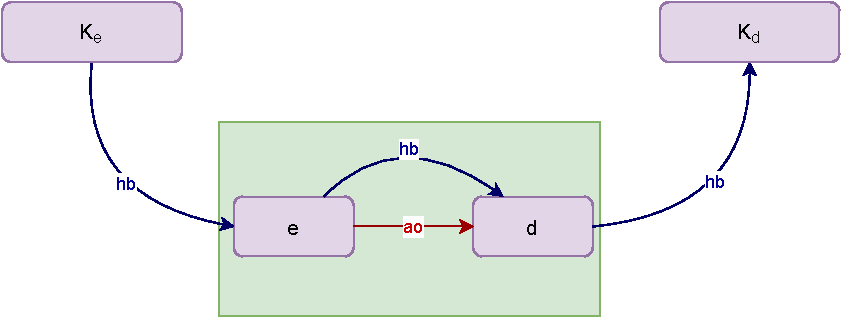
\includegraphics[scale=0.7]{Q1(a).pdf}
            \caption{For any Candidate Execution of $C$, the set $K_e$ and $K_d$}
            \label{fig:my_label}
        \end{figure}
        
        The idea is that if these relations are intact, then the relations among events from the first and second set will also hold due to transitivity.
        
        To ensure this, firstly note that in terms of direct happens-before relations, on reordering, any $Candidate Execution$ of $C$ will have the following changes
        
        %Show a figure here 
        \begin{figure}[H]
            \centering
            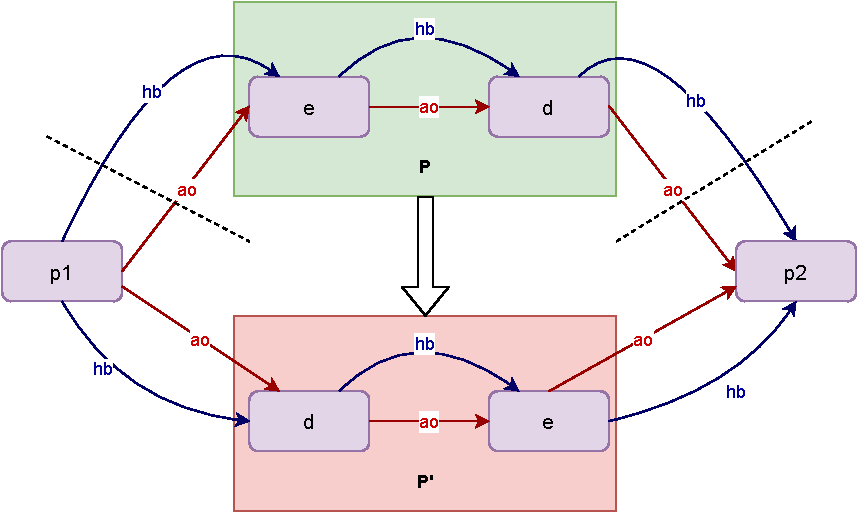
\includegraphics[scale=0.7]{Q1(b).pdf}
            \caption{The direct relation changes that can be observed while reordering events $e$ and $d$}
            \label{fig:my_label}
        \end{figure}
        
        The figure above is to show that, for any $Candidate Execution$ of $C$, the following is true
        \[
            cons(p1,e) \wedge dir(p1,e) \wedge dir(e,d) \wedge cons(d,p2) \wedge dir(d,p2)
        \]
        
        and for that of $C'$,
        \[
            cons(p1,d) \wedge dir(p1,d) \wedge dir(d,e) \wedge cons(e,p2) \wedge dir(e,p2) 
        \]
        
        Note that here, $p1$ and $p2$ are part of the respective sets of events $K_e$ and $K_d$. So we have the following relations that we need to preserve w.r.t these two events
        
        \[
            \reln{p1}{hb}{e} \wedge \reln{p1}{hb}{d} \wedge \reln{d}{hb}{p2} \wedge \reln{e}{hb}{p2}
        \]
        
        After reordering, we do have these relations preserved due to transitivity
        
        \[
            \reln{p1}{hb}{d} \ \wedge \ \reln{d}{hb}{e} \ \Rightarrow \ \reln{p1}{hb}{e}
        \]
        \[
            \reln{e}{hb}{p2} \ \wedge \ \reln{d}{hb}{e} \ \Rightarrow \ \reln{d}{hb}{p2}
        \]
        \[
            \reln{p1}{hb}{d} \ \wedge \ \reln{d}{hb}{e} \ \wedge \ \reln{e}{hb}{p2} \ \Rightarrow \ \reln{p1}{hb}{p2}
        \]
        
        \critic{blue}{When $e$ is the first event or $d$ is the last event, assume a dummy event that can act as $p1$ and $p2$ having the same relations.}
        
        %Put a figure here to show that perhaps
        
        %If we take specific cases where $e$ is the first event and $d$ is the last event in the agent, the above change in relation may not be there as events $p1$ or $p2$ may not exist. An example where $e$ is the first event is shown below:
        
        %Show a figure here
        %\begin{figure}[H]
         %   \centering
          %  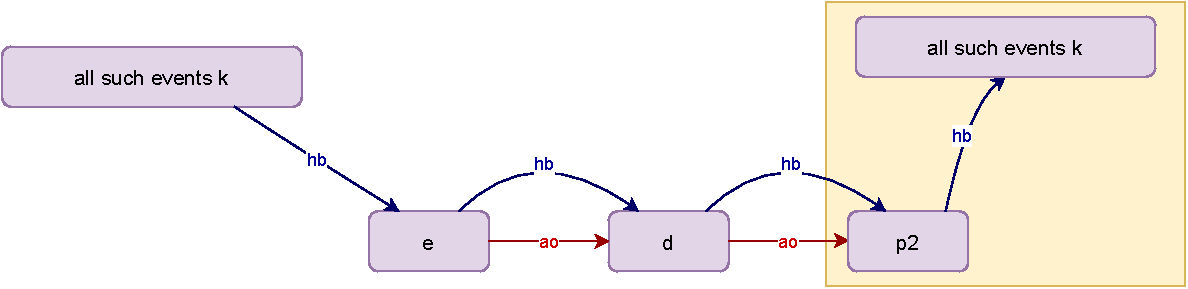
\includegraphics[scale=0.7]{Q1(c).pdf}
           % \caption{Caption}
        %    \label{fig:my_label}
        %\end{figure}
        
        If we can "pivot" the remaining set $K_e$ to $p1$ and $K_d$ to $p2$, it would ensure that our intended relations remain intact after reordering by transitivity. To state formally, we have a valid pair of pivots $<p1,p2>$ when 
        
        \[
            \forall \ k \in K_e-\{p1\}, \ \reln{k}{hb}{p1} 
        \]
        
        \[
            \forall \ k \in K_d - \{p2\}, \ \reln{p2}{hb}{k}
        \]
        
        %Show a figure here
        \begin{figure}[H]
            \centering
            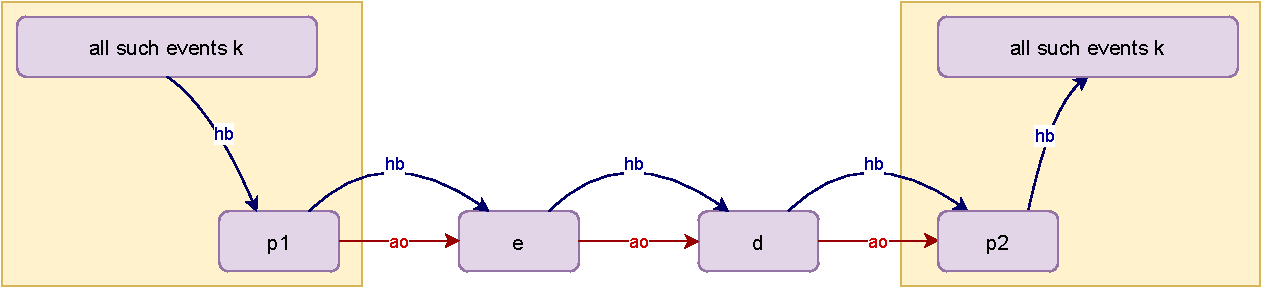
\includegraphics[scale=0.7]{Q1(d).pdf}
            \caption{For any Candidate execution, the intuition behind valid pivots $<p1,p2>$}
            \label{fig:my_label}
        \end{figure}
        
        
        By lemma 1, we have for $C$, the following condition where $p1$ is a valid pivot
        
        \[
            \et{e}{uo} \vee (\et{e}{sc} \wedge \event{e}{W})
        \]
        
        Similarly, by lemma 2, we have for $C$, the following condition where $p2$ is a valid pivot
        
        \[
            \et{d}{uo} \vee (\et{d}{sc} \wedge \event{d}{R})
        \]
        
        The following table summarizes the cases where we have a valid pair of pivots $<p1,p2>$
        %Show a general table here 
        \begin{figure}[H]
            \centering
            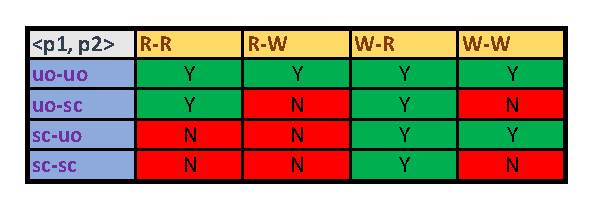
\includegraphics[scale=0.7]{Table1_Final.pdf}
            \caption{Table summarizing whether we have valid pair of pivots based on  $e$ and $d$}
            \label{fig:my_label}
        \end{figure}
        
        %In terms of the special cases when $e$ is the first event or $d$ is the last event in the agent, checking if valid pivots exist may not be possible. 
        
        %If we however, place \textit{dummy} events $pd1$ and $pd2$ before the first event and after the last event. We are ensured that there is a possibility of a pivot.
        
        %SHow figure here of dummy events attached before $e$ when $e$ is the first event.
        
        %Show a figure where  e is the first event, but d is not the last. But p2 is not a valid pivot, so we can eliminate the case.
        
        %CHange this figure to dummy event
        %\begin{figure}[H]
        %    \centering
        %    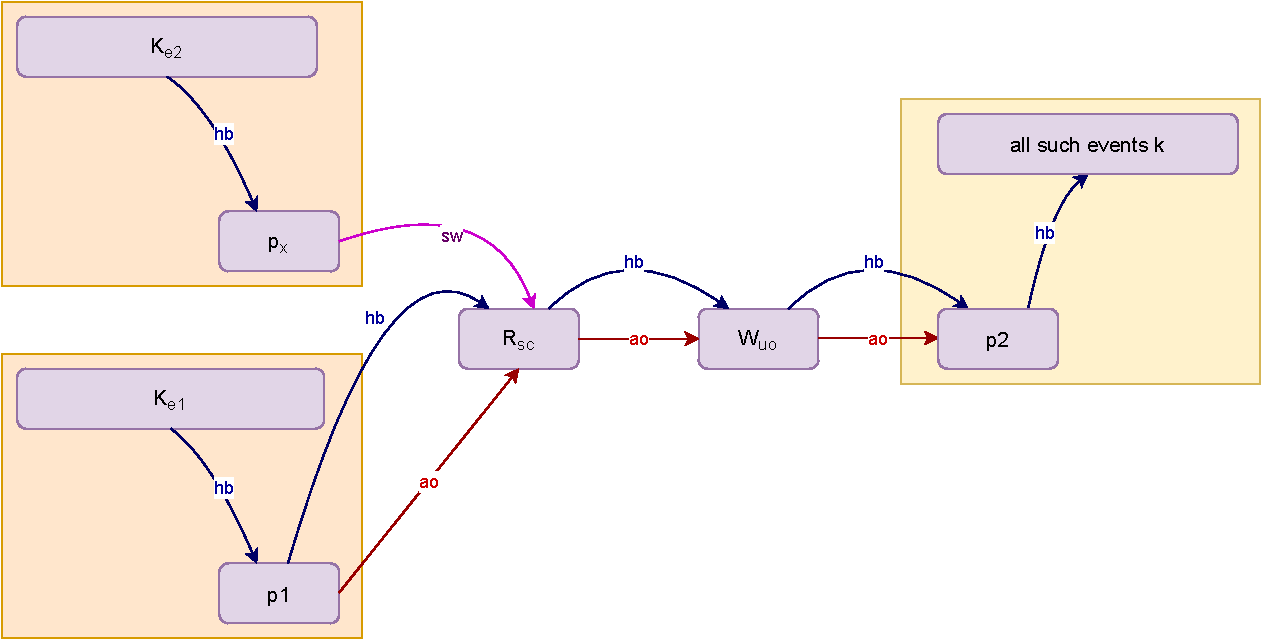
\includegraphics[scale=0.7]{Q1(e).pdf}
        %    \caption{Caption}
        %    \label{fig:my_label}
        %\end{figure}
        
        %For such cases, it is important to note what exactly the two sets of $k$ are in $P$. In the case where $e$ is the first event, the first set would consist of those events $k$ which lack an agent-order relation with $e$. However, note that this set maintains the same relation with $e$ in $P'$, irrespective of event $d$. This is because there is a direct \textit{synchronize-with} relation with one of the elements from the first set and $e$, which remains unchanged, if it existed in $P$.  
        
        %ARE THESE TWO FIGURES REQUIRED? IF so Change them
        
        We show a simple example where we do not have a valid pair of pivots, particularly because $p1$ is not a valid pivot. Note that in this example, $K_e = K_{e1} + K_{e2} + p1 + p_x$
        %Show figure here of program P
        \begin{figure}[H]
            \centering
            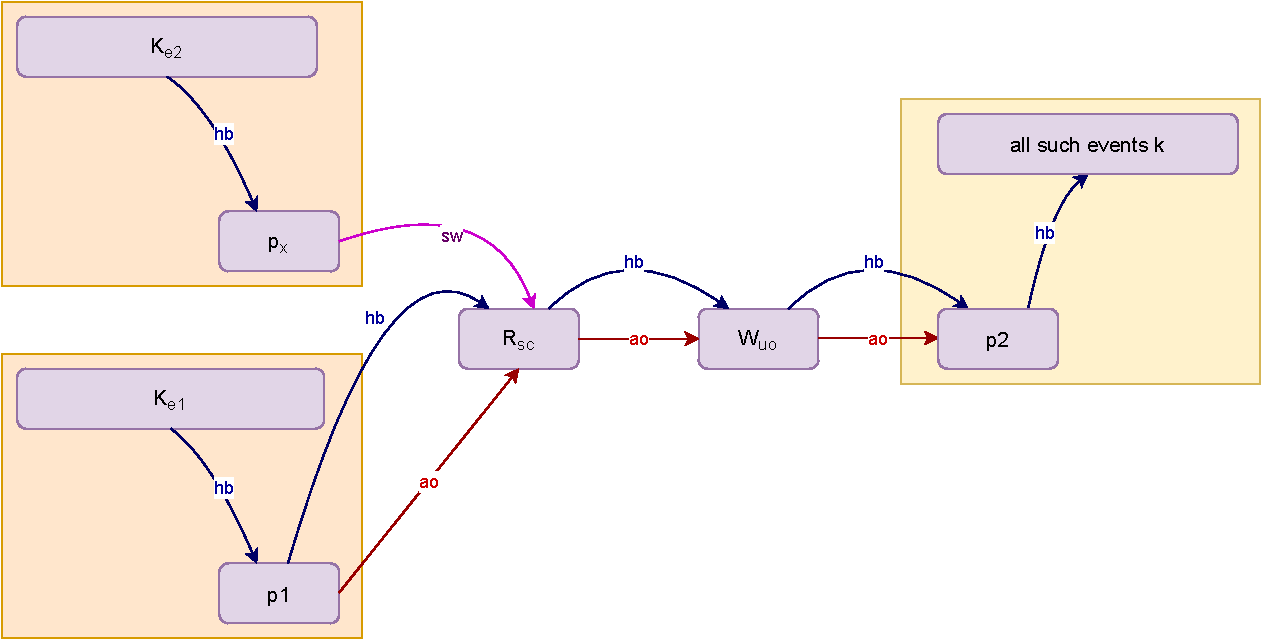
\includegraphics[scale=0.7]{Q1(e).pdf}
            \caption{A Candidate Execution where p1 is not a valid pivot}
            \label{fig:my_label}
        \end{figure}
        
        %Show figure here of program P'
         \begin{figure}[H]
            \centering
            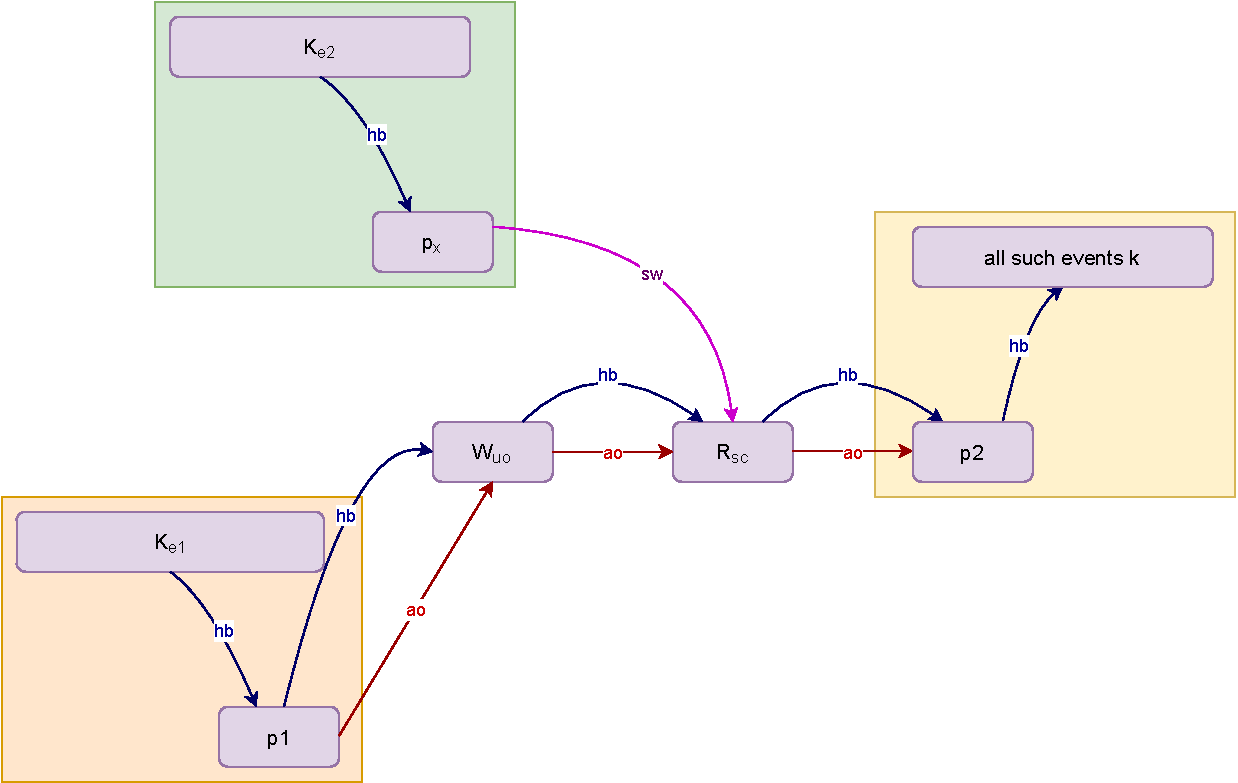
\includegraphics[scale=0.7]{Q1(f).pdf}
            \caption{The resultant Candidate Execution after reordering, exposing the relations with $p_x$, $K_{e2}$ and $d$ that are lost}
            \label{fig:my_label}
        \end{figure}
        
        
        %Give excel sheet figure for question 1 in the most general case
        %Give excel sheet figure for when $e$ is the first event
        %Give excel sheet figure for when $d$ is the last event
        
        %It cannot be the first question to address, because from the first question we get the set of $k$ preserved. This question would establish the link from the first to the second while ensuring relations with e and d remain intact.
        
        %MAKE SOME MAJOR CHANGES TO THIS
        \paragraph{2. Additional \textit{happens-before} relations}
        Although we have identified the cases when \textit{happens-before} relations are preserved, we also get some additional relations in some of them.
        
        %Show an example here and explain
        As an example, for the case when $d$ is a sequentially consistent read, by lemma 1, in any execution of $C$
        
        \[
            \reln{k}{hb}{d} \centernot\Rightarrow \reln{k}{hb}{e} 
        \]
        
        But in $Executions$ of candidate $C'$, by transitivity, we have 
        \[
            \reln{k}{hb}{d} \Rightarrow \reln{k}{hb}{e} 
        \]
        
        This is because, there are sets of relations that come through certain \textit{synchronize-with} relations. Thus, although we are able to preserve relations that existed in any $Candidate Execution$ of $C$, we also in the process, introduce new ones in $Candidate Executions$ of $C'$. The figure below shows pictorially an example of a Candidate Execution of $C$ for the case above 
        
        %Show figure here of program P 
        \begin{figure}[H]
            \centering
            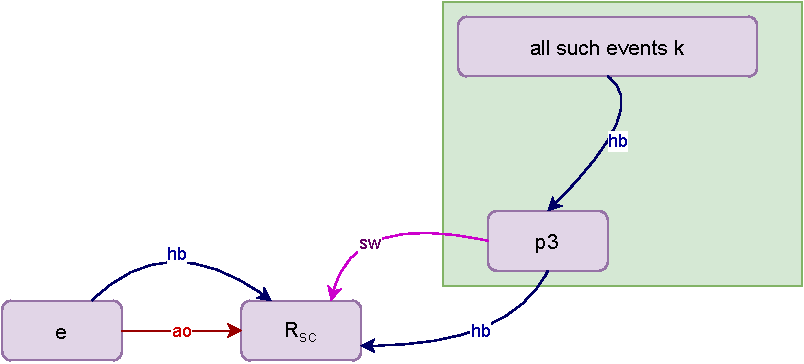
\includegraphics[scale=0.7]{Q2(c).pdf}
            \caption{A Candidate Execution where $d$ is a sequentially consistent read}
            \label{fig:my_label}
        \end{figure}
        
        %Show figure here of program P'
        \begin{figure}[H]
            \centering
            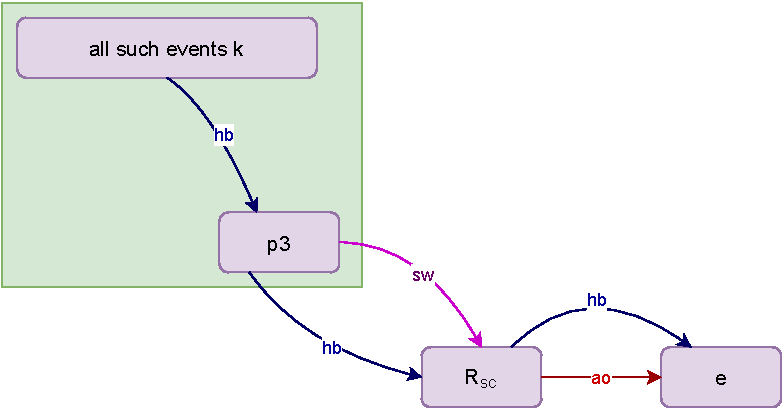
\includegraphics[scale=0.7]{Q2(d).pdf}
            \caption{The Candidate Execution after reordering, exposing the new relations established with $e$, $p3$ and set $k$}
            \label{fig:my_label}
        \end{figure}
        
       
       
        %To identify the cases when this is true, notice that by transitive property, in program $P$, all  \textit{happens-before} relations that come to $e$ go to $d$ and all such relations that go from $d$ also go from $e$. In program $P'$, the same implication would be answering the questions whether all \textit{happens-before} relations that come to $e$ go through $d$ and whether all relations that go from $d$ go from $e$. 
        
        %Show figure for the first question in both program P and P'
        %\begin{figure}[H]
         %   \centering
         %   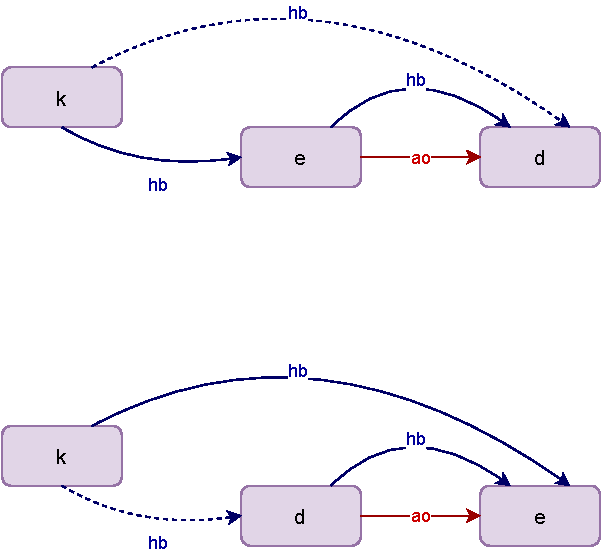
\includegraphics[scale=0.7]{Q2(a).pdf}
         %   \caption{Caption}
         %   \label{fig:my_label}
        %\end{figure}
        
        %Show figure for the second questions in both program P and P'
        %\begin{figure}[H]
        %    \centering
        %    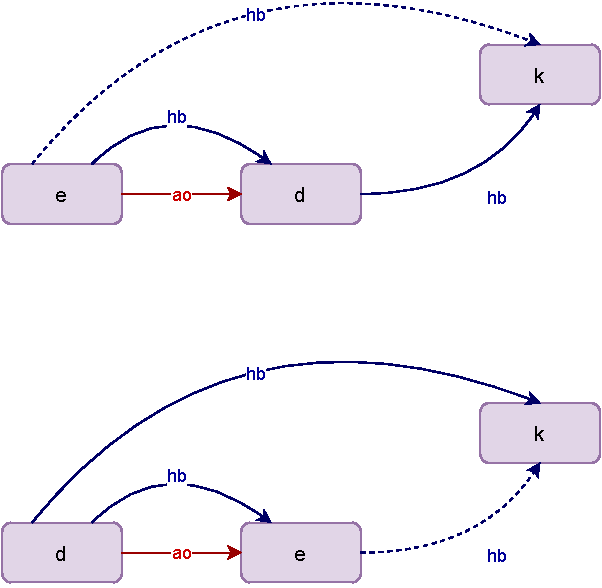
\includegraphics[scale=0.7]{Q2(b).pdf}
        %    \caption{Caption}
        %    \label{fig:my_label}
        %\end{figure}
        
      
        To summarize, the table below shows the cases where new relations could be introduced. 
        %Show the table here
        \begin{figure}[H]
            \centering
            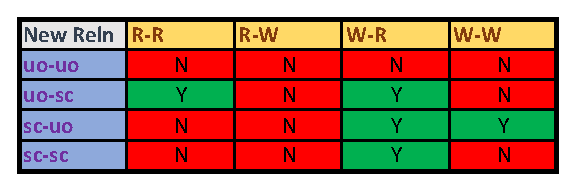
\includegraphics[scale=0.7]{Table2_Final.pdf}
            \caption{Table summarizing when new \textit{happens-before} relations could be introduced based on having valid pair of pivots }
            \label{fig:my_label}
        \end{figure}

        For these cases, we must know whether these new relations introduce new observable behaviors. 
        
        %Needs a few major changes and tables split cases into disjoint, overlapping and equal ranged events 
        \paragraph{3. Do new relations introduce new observable behaviors?}
        In any candidate execution, reordering events $e$ and $d$ eliminate the relation $\reln{e}{hb}{d}$ and introduce the new relation $\reln{d}{hb}{e}$. If this new relation itself could bring about new behaviors, we need not consider other new relations introduced in the process. 
        
        To analyze this, notice that the axiom of \textit{Coherent Reads} and that of \textit{Sequentially Consistent Atomics} use $\stck{_{hb}}$ relations to place restrictions on $\stck{_{rf}}$. These are subject to the relation between the ranges of events involved. So, if we divide the cases we have based on $e$ and $d$ having disjoint, overlapping or equal ranges, we can summarize when these two axioms could play a role in allowing a new behaviour to occur.
        
        %SHow the three tables here
        \begin{figure}[H]
            \centering
            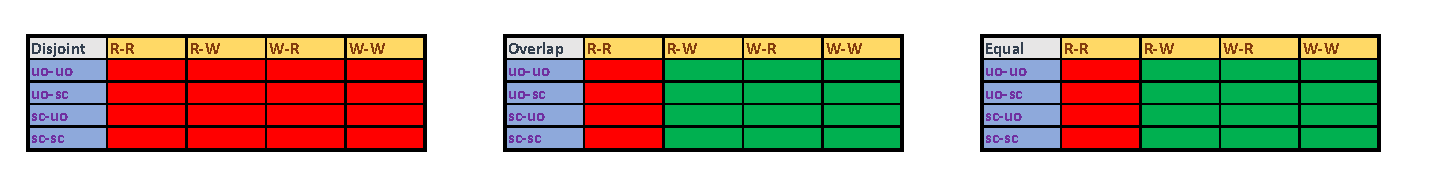
\includegraphics[scale=0.7]{Table_Range.pdf}
            \caption{Cases based on the ranges of $e$  and $d$ where the axiom of Coherent Reads / Sequentially Consistent atomics can apply to introduce new observable behaviors on reordering}
            \label{fig:my_label}
        \end{figure}
        
        
        Notice that only when both $e$ and $d$ are reads, the relation of range in which they operate is irrelevant for any axiom to play a role. Whereas, in other cases, overlapping and equal ranges, the axioms do play a role.
        
        
        For the other additional relations that are established, we can divide them into 5 cases. 
        %Show a figure here summarizing the four cases
        \begin{figure}[H]
            \centering
            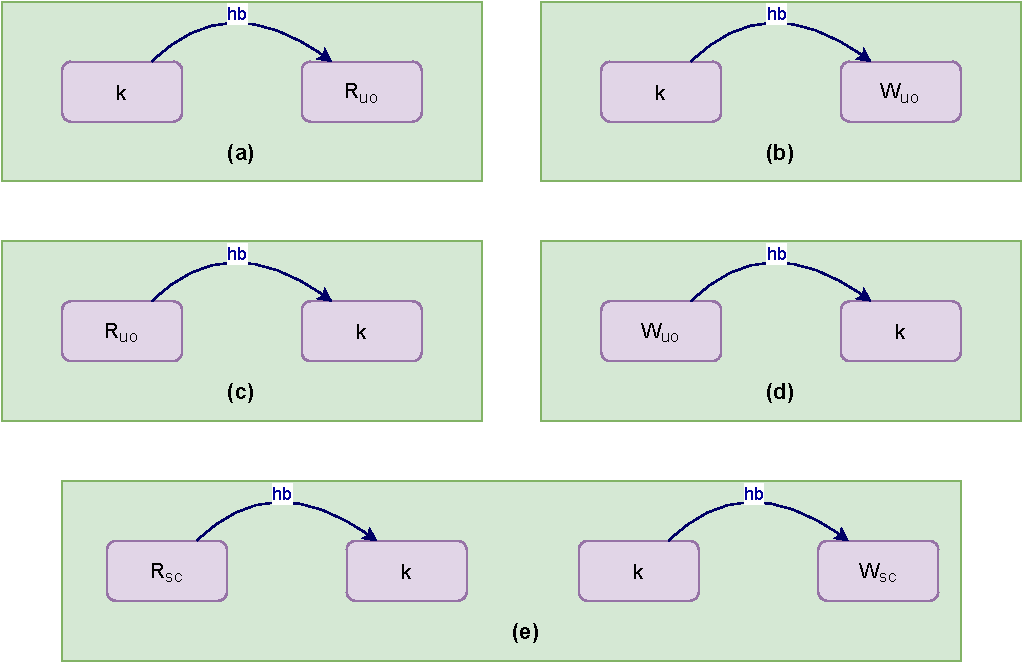
\includegraphics[scale=0.7]{Q3(a).pdf}
            \caption{Caption}
            \label{fig:my_label}
        \end{figure}
        
        In each of the above cases, note firstly that we need to only consider cases where their ranges are overlapping/equal.
        
        %Addressing the first case. 
        In the first case (a), depending on what event $k$ is, we would have the following cases where the axioms would play a role. 
        
        %Show all cases here for different k
        \begin{figure}[H]
            \centering
            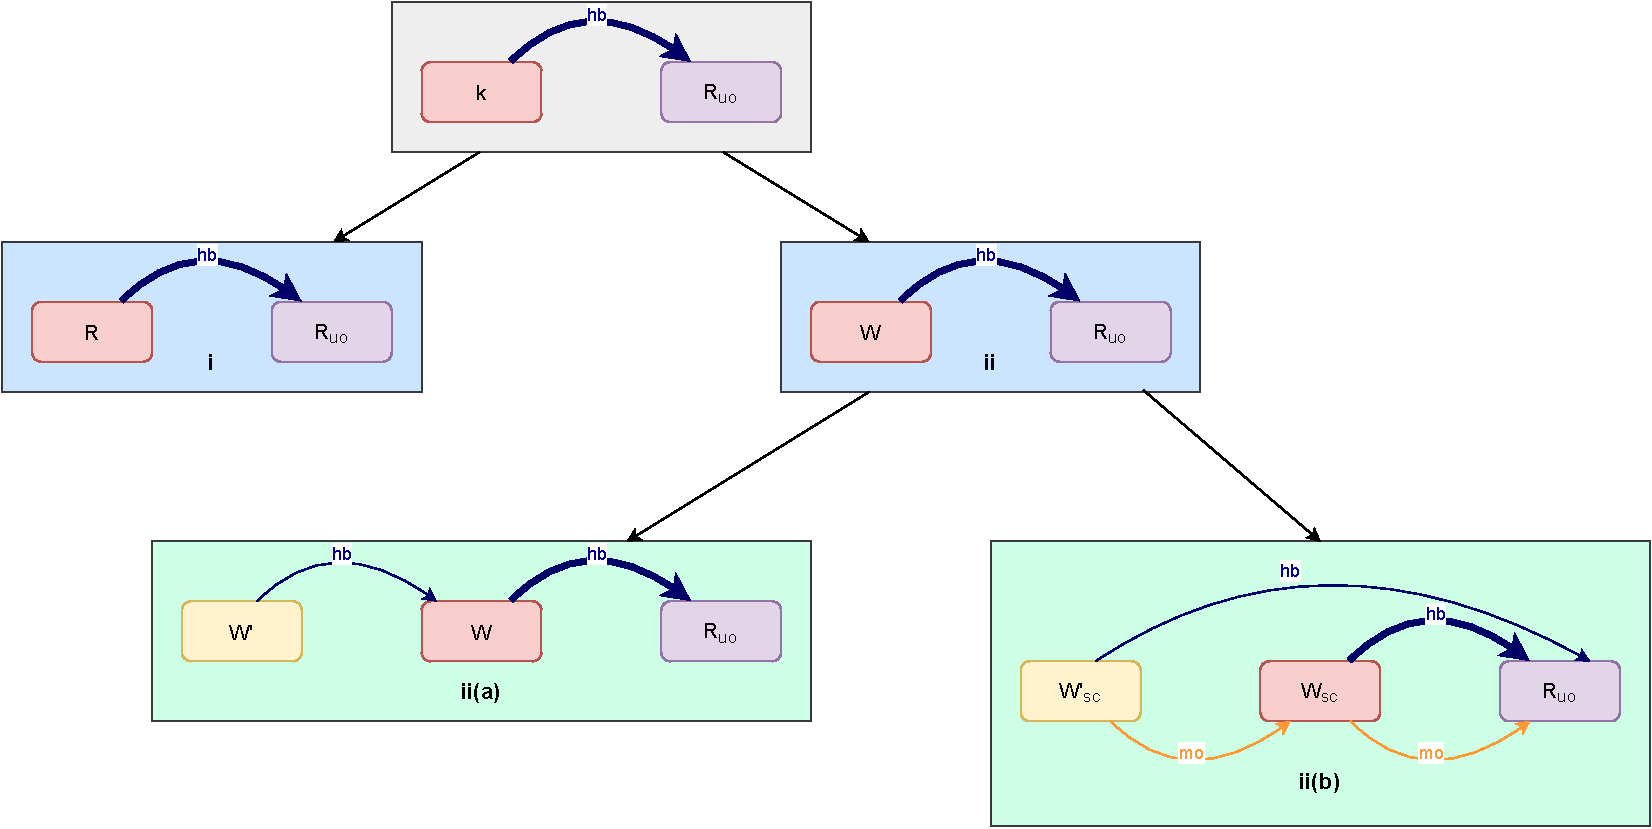
\includegraphics[scale=0.6]{Q3_(b)Case1.pdf}
            \caption{The role of the axioms on introducing a new relation between an unordered Read and some event $k$}
            \label{fig:my_label}
        \end{figure}
        
        %Might have to elaborate this more
        \begin{enumerate}
            \item For subcase (i), none of the axioms have any implications on observable behaviors.
            \item For subcase (iii), the axiom of coherent reads could in restrict $R$ from reading overlapping ranges of $W'$ with $W$.
            \item Subcase (iv) restricts R from reading $W'$ by the axiom of sequentially consistent atomics if $W$ and $W'$ have equal ranges. 
        \end{enumerate}
        
        The other cases, also have instances which can satisfy some cases of the axioms, thus restricting possibly some $\stck{_{rf}}$ relations.
        
        \begin{figure}[H]
            \centering
            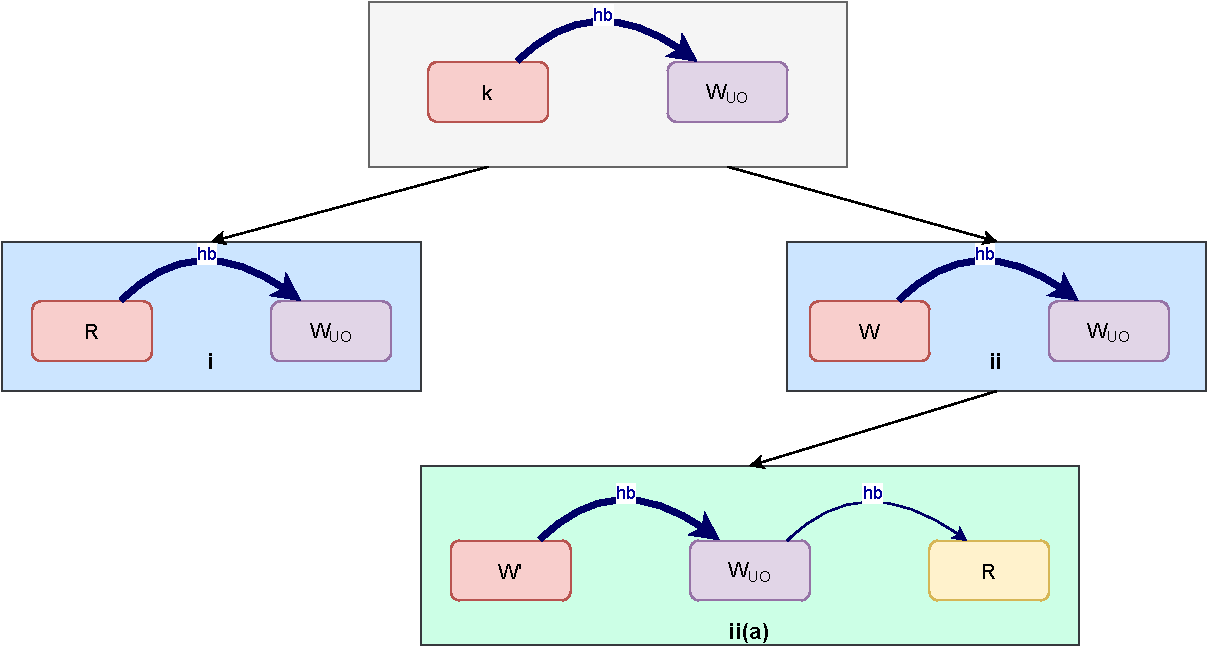
\includegraphics[scale=0.6]{Q3_(c)Case2.pdf}
            \caption{(i) and (ii(b)) satisfy the axiom of Coherent Reads}
            \label{fig:my_label}
        \end{figure}
          
          
        \begin{figure}[H]
            \centering
            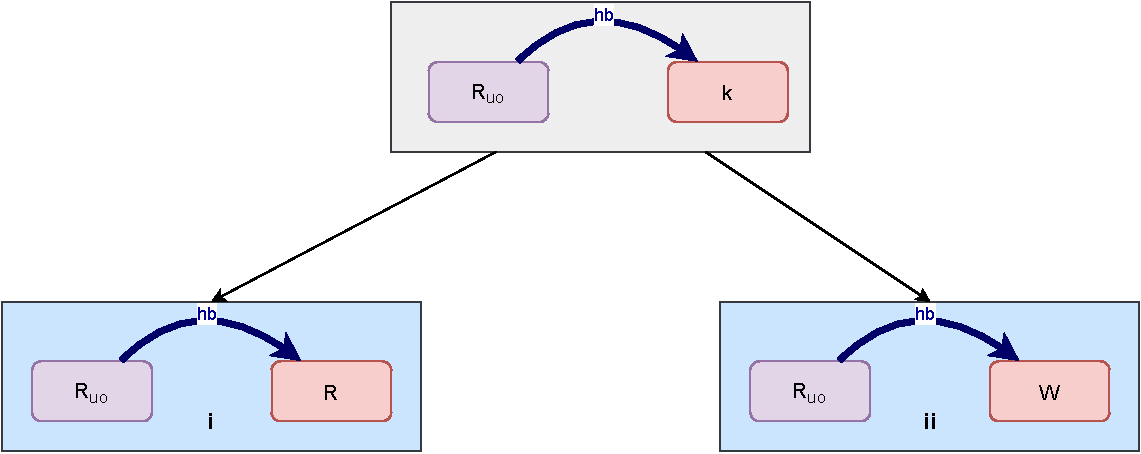
\includegraphics[scale=0.6]{Q3_(d)Case3.pdf}
            \caption{(ii) satisfies the axiom of Coherent Reads}
            \label{fig:my_label}
        \end{figure}
        
        
        \begin{figure}[H]
            \centering
            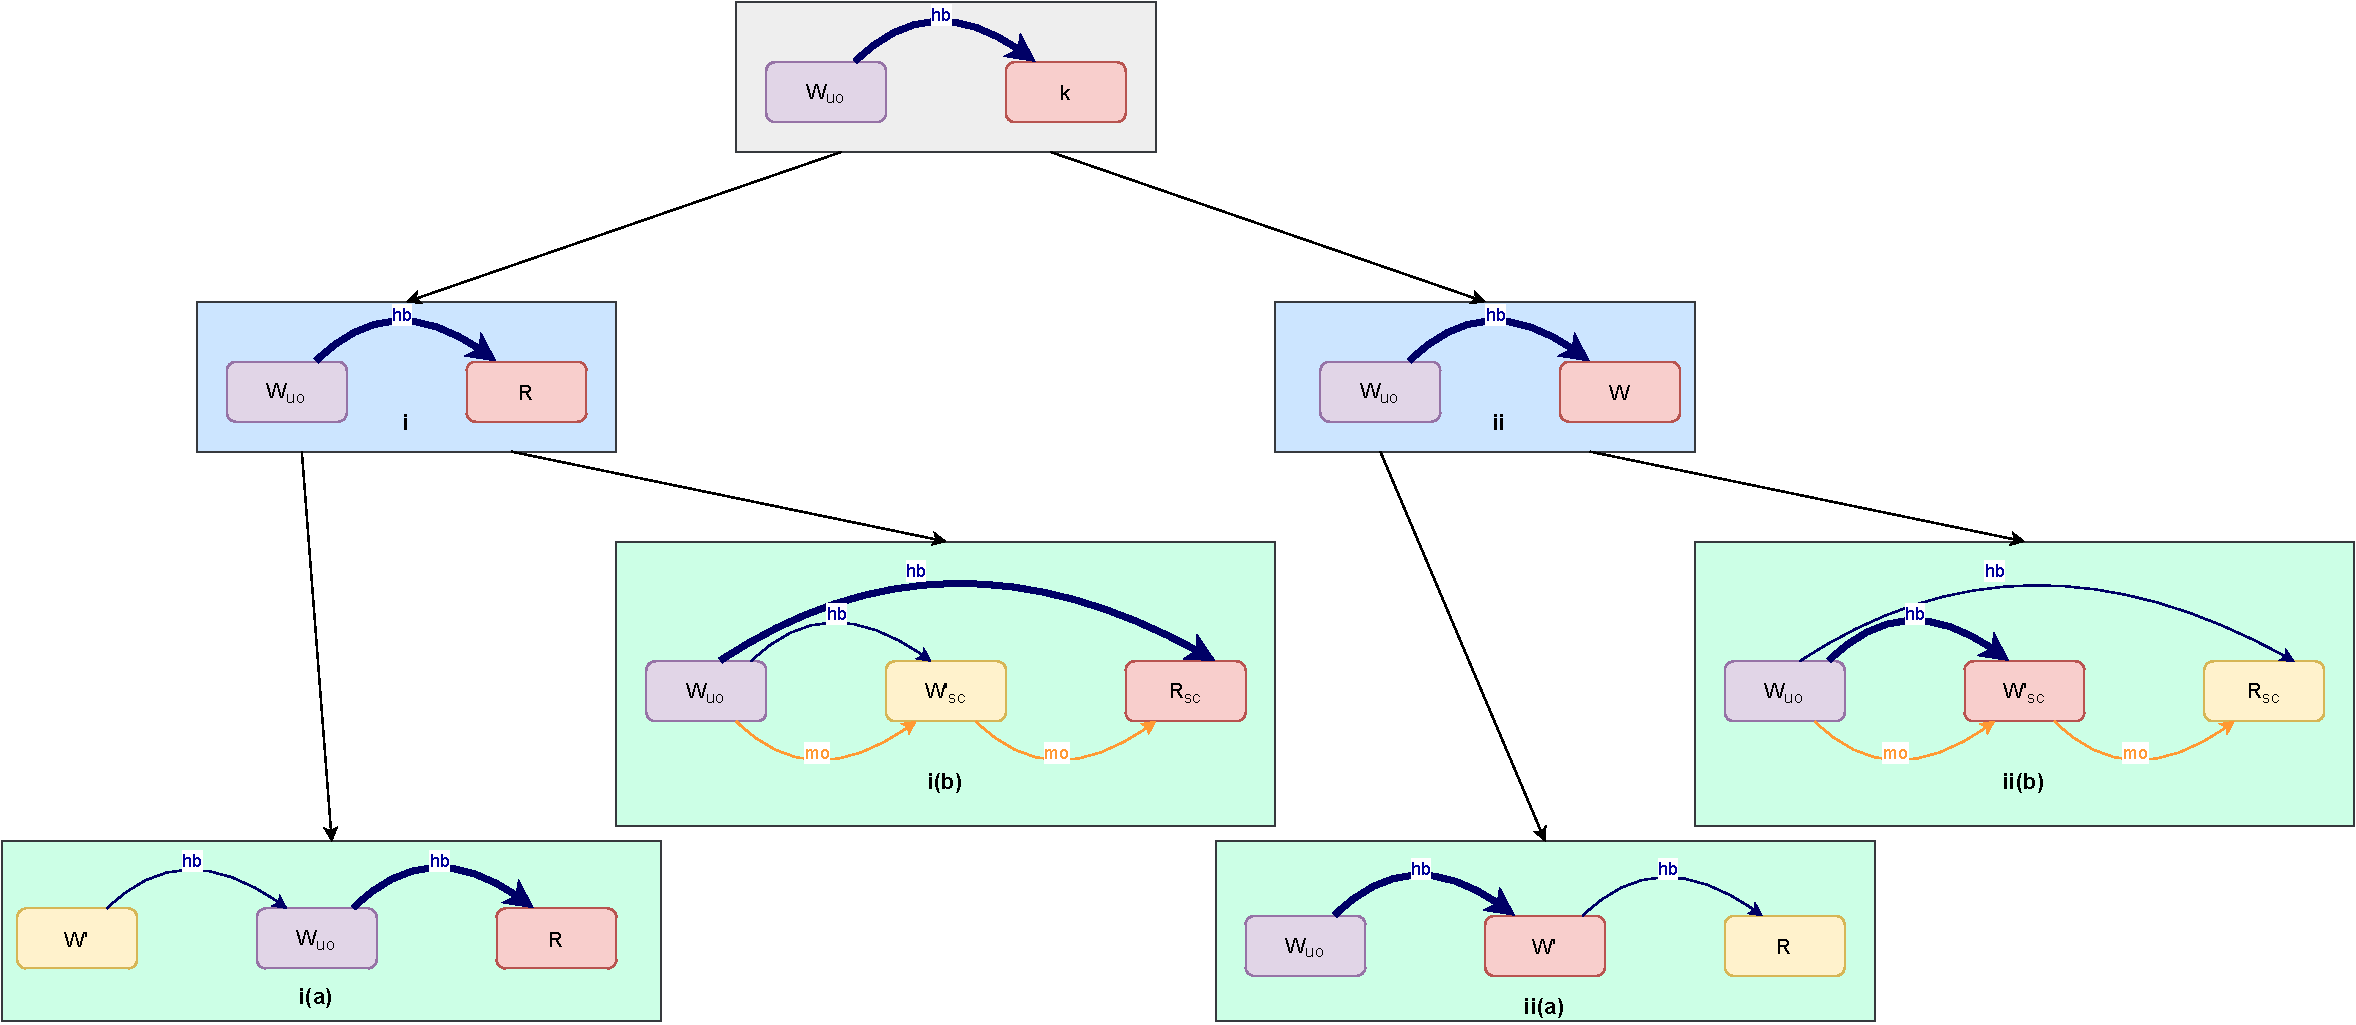
\includegraphics[scale=0.4]{Q3_(e)Case4.pdf}
            \caption{(i(a)), (ii(a)) satisfy the axiom of Coherent Reads, whereas (i(b)), (ii(b)) satisfy the axiom of Sequentially Consistent Atomics}
            \label{fig:my_label}
        \end{figure}
        
        The last case (v) is a repetition of cases of the above. The main point is to note that satisfying these particular axioms implies a restriction of $\stck{_{rf}}$ relation among events. Note also that without this new relation, these conditions for these axioms wouldn't have been satisfied. Thus, this implies that we are only possibly reducing the observable behaviors of any Candidate Execution. 
        %Show the rest of the figures
        
        \critic{blue}{The main reason for this is that these axioms are defined restricting \textit{reads-from} relations. So in any case where adding an additional \textit{happens-before} relation "triggers" an axiom, we are bound to have some behaviors restricted. It is this fact that is elicited explicitly by going case wise on all relations that are introduced.}
        
        \paragraph{4. Presence of cycles?}
        Though it may seem the previous questions have answered all our concerns to ensure set of observable behaviours shown by $Executions$ of $C'$ is a subset of $C$, we have not addressed whether the additional relations introduce any \textit{happens-before} cycles. Consider the example of relations with three events below. 
        
        \begin{figure}[H]
            \centering
            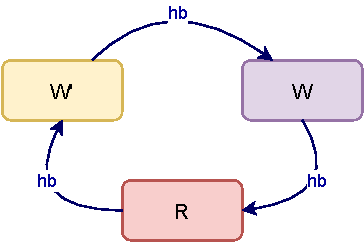
\includegraphics[scale=0.7]{Q4(a).pdf}
            \caption{Caption}
            \label{fig:my_label}
        \end{figure}
        
        Notice that here, the axiom of coherent reads restricts $R$ to read from $W'$.
        
        \[
            \reln{R}{hb}{W'} \Rightarrow \neg \reln{R}{rf}{W'}
        \]
        
        But by transitive property, it is also the case that $\reln{W'}{hb}{R}$. 
        
        \[
            \reln{W'}{hb}{W} \ \wedge \ \reln{W}{hb}{R} \ 
            \Rightarrow \ 
            \reln{W'}{hb}{R}
        \]
        
        As per this, the axiom of coherent reads shouldn't restrict $\reln{R}{rf}{W'}$. To avoid such cases, we will need to ensure that no Candidate Execution of $C'$ after $e$ and $d$ are reordered have $\stck{_{hb}}$ cycles. For our purpose, we assume the Candidate Executions of $C$ contain no such cycles. 
        
        Note that if a cycle exists after reordering, then 
        \begin{enumerate}
            \item The relations preserved do not themselves create a cycle
            \item Additional new relations may introduce cycles
        \end{enumerate}
       
        The first part is straightforward as we assume we can only do reordering on Candidate Exectuions of $C$ not having cycles. 
        
        To address the second part, we first address the cases where $\reln{d}{hb}{e}$ may be part of the cycle. The other event $k$, may be either from the set $K_e$, $K_d$ or a new relation that is formed.
        
        %Show figure here
        \begin{figure}[H]
            \centering
            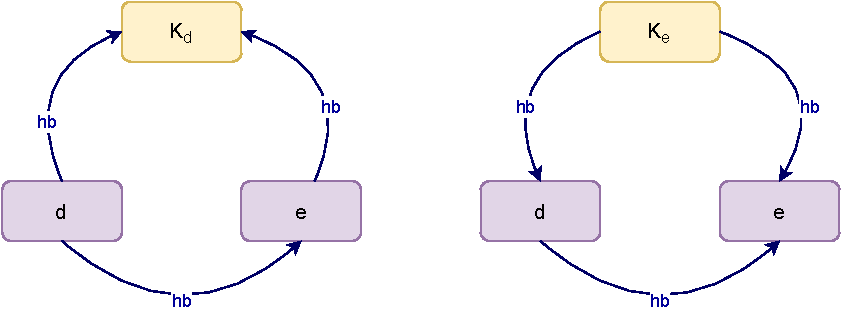
\includegraphics[scale=0.7]{Q4(a)_1.pdf}
            \caption{If k belongs to one of the sets $K_e$ or $K_d$}
            \label{fig:my_label}
        \end{figure}
        
        The above figure shows that $k$ cannot belong to either of the sets, as their relations with $e$ and $d$ will not result in a cycle. 
        
        For cases where $\reln{k}{hb}{e}$ is the set of new relations, note that by lemma 1
        \[
            \reln{k}{hb}{e} \Rightarrow \reln{k}{hb}{d}
        \]
        
        
        For cases where $\reln{d}{hb}{k}$ is the set of new relations, by lemma 2
        \[
            \reln{d}{hb}{k} \Rightarrow \reln{e}{hb}{k}
        \]
        
        So for both these cases also, a cycle with $\reln{d}{hb}{e}$ does not exist. The following figure shows pictorially this fact. 
        
        %Show figure here
        \begin{figure}[H]
            \centering
            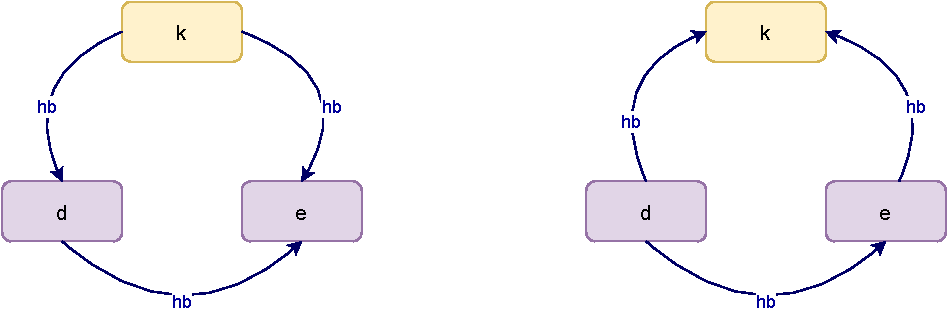
\includegraphics[scale=0.7]{Q4(a)_2.pdf}
            \caption{If $\reln{k}{hb}{e}$ or $\reln{d}{hb}{k}$ are new sets of relations}
            \label{fig:my_label}
        \end{figure}
        
        
        For the one case where we have two new sets of relations formed, i.e $\reln{d}{hb}{k}$ and $\reln{k}{hb}{e}$, we could have a case where $k$ is a common event for both sets. But, by lemma 1, we also have $\reln{k}{hb}{d}$ and by lemma 2, $\reln{e}{hb}{k}$. Thus, we have a cycle. 
        
        %Show figure here
        \begin{figure}[H]
            \centering
            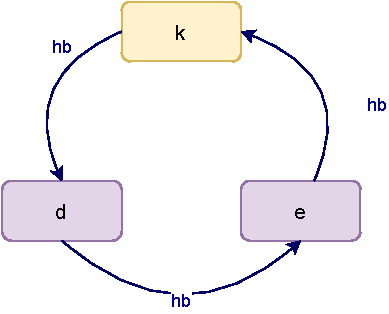
\includegraphics[scale=0.7]{Q4(a)_3.pdf}
            \caption{A cycle exists in the case where we have two new sets of relations ($\reln{k}{hb}{e}$ and $\reln{d}{hb}{k}$) }
            \label{fig:my_label}
        \end{figure}
        
        Now for the case when $\reln{d}{hb}{e}$ may not be part of the cycle, we have only two other relations, $\reln{k}{hb}{e}$ or $\reln{d}{hb}{k}$.
        
        Considering the first scenario where the new set of relations are of the form $\reln{k}{hb}{e}$. Suppose a cycle exists with another event $k'$
        
        \[
            \reln{k}{hb}{e} \ \wedge \
            \reln{e}{hb}{k'} \ \wedge \
            \reln{k'}{hb}{k}
        \]
        
        Note that the latter two relations are not new, since the only new set of relations are of the first form. Now, by lemma 1
        
        \[
            \reln{k}{hb}{e} \Rightarrow \reln{k}{hb}{d}
        \]
        
        So, the following is also a cycle
        \[
            \reln{k}{hb}{d} \ \wedge \
            \reln{e}{hb}{k'} \ \wedge \
            \reln{k'}{hb}{k}
        \]
        
        But these relations already exist in the original Candidate Execution, which implies a cycle existed before reordering. This contradicts our assumption that we only reorder when the Candidate Executions of $C$ have no cycles. Thus, by contradiction such a cycle cannot exist.
        
        In similar lines for the cases where the set of new relations are of the form $\reln{d}{hb}{k}$, we can show by contradiction that a cycle cannot exist. 
        
        The table below summarizes the valid cases where, we have a pair of valid pivots, where new relations do not introduce new observable behaviors and do not have cycles. 
        %Show the table here
        \begin{figure}[H]
            \centering
            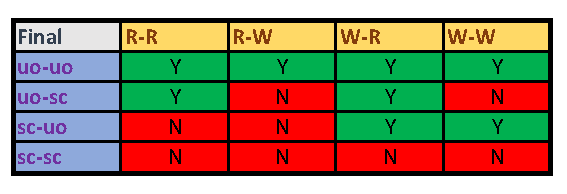
\includegraphics[scale=0.7]{Table4_Final.pdf}
            \caption{The final table summarizing the valid cases where observable behaviors will only be a subset after reordering.}
            \label{fig:my_label}
        \end{figure}
    
        The table above, precisely is the definition of a reorderable pair. 
        
        \critic{blue}{Keep in mind that the comparision of ranges is done while addressing question 3 in the proof, so the table above, implicitly also takes into account only the valid cases where ranges are also correct}
        
\end{proof}

\begin{corollary}
    Consider a Candidate C of a program and its Candidate Executions which are valid. Consider two events $e$ and $d$ such that $\neg \cons{e}{d}$ is true in C and $\reln{e}{ao}{d}$. Consider another Candidate C' resulting after reordering $e$ and $d$ in C. Then, the set of Observable behaviors possible in C' is a subset of C only if $Reord(e,d)$ and the following holds true.
    
    \[
        \forall \ k \ \textit{s.t.} \ 
        \reln{e}{ao}{k} \ \wedge \ \reln{k}{ao}{d} \ . \ 
        Reord(e,k) \ \wedge \ Reord(k,d)
    \]
    
\end{corollary}
    
\begin{proof}
    
\end{proof}
    
\subsection{Counter examples for the invalid cases}

\subsection{}

    

    
    
    
    
    